\section{Introduction}
\label{sec:intro}

\begin{figure}[ht]
    \centering
    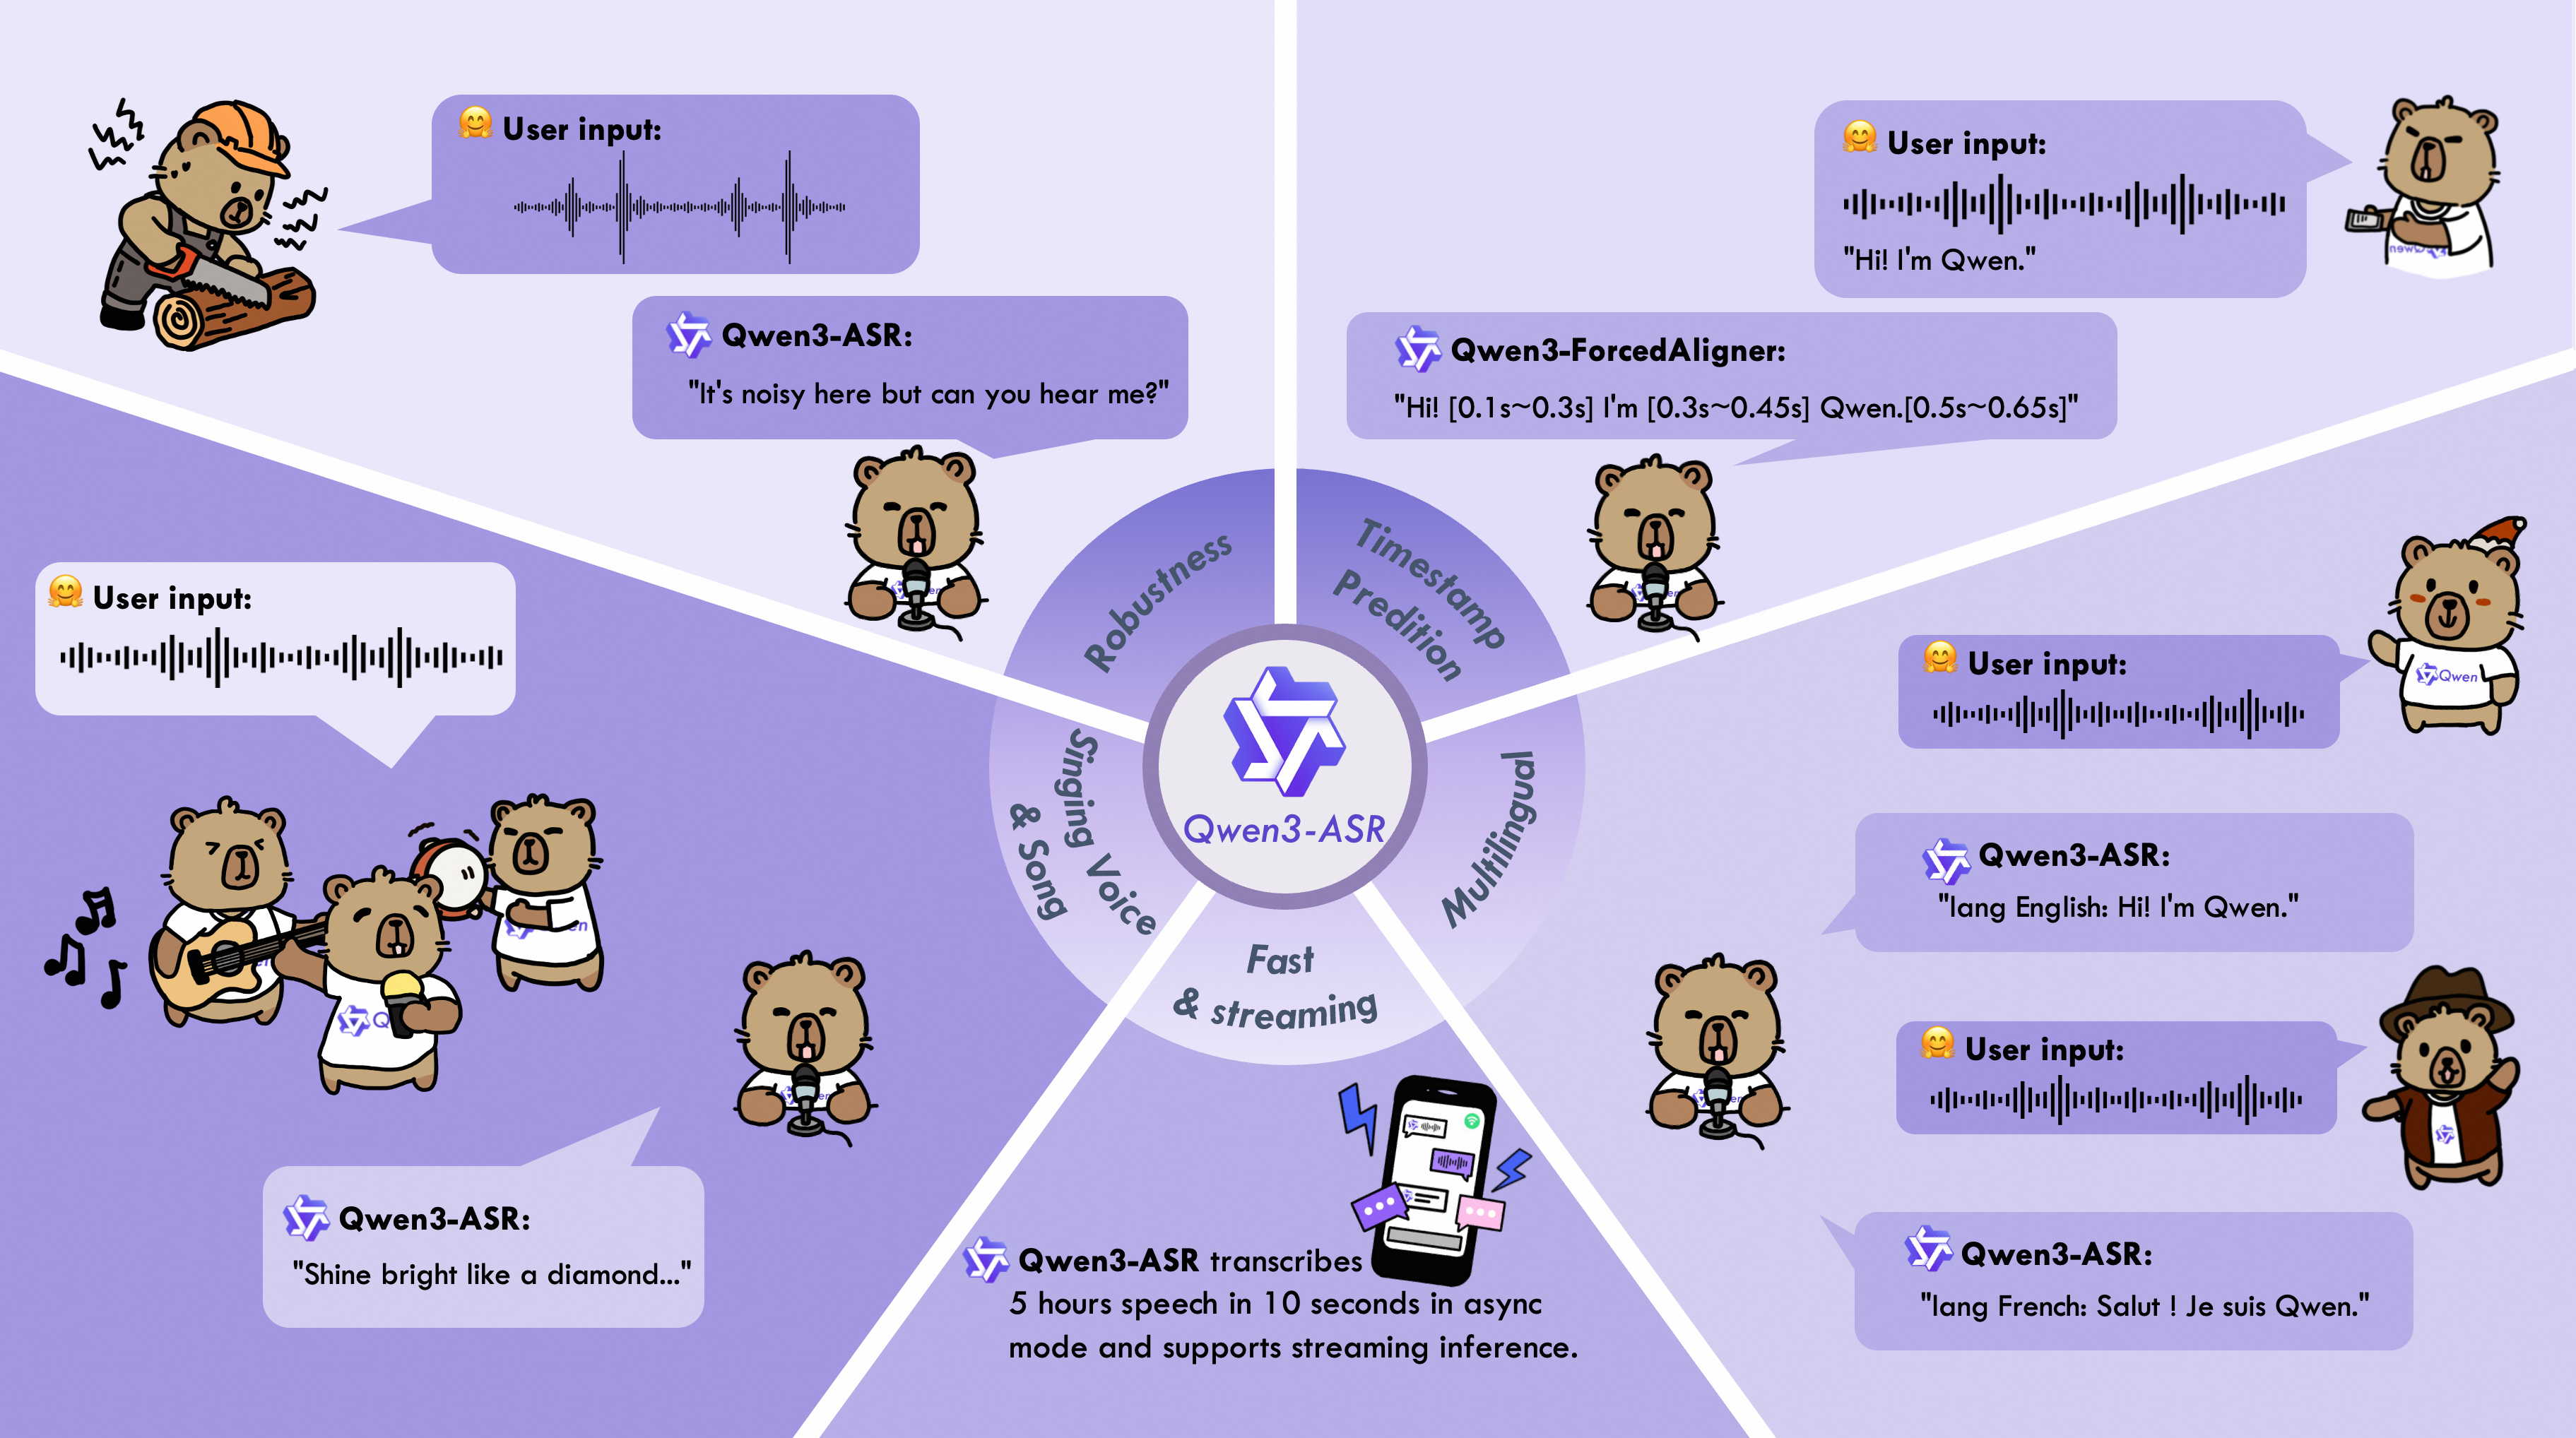
\includegraphics[width=\linewidth]{figures/qwenasr-intro.png}
    \caption{Qwen3-ASR family includes all-in-one ASR models with advantages in multilingual, noisy speech recognition, singing voice recognition and inference efficiency, so as to a novel multilingual speech forced alignment model for predicting timestamps of words or sentences in ASR results.}
    \label{fig:placeholder}
\end{figure}

In recent years, Automatic Speech Recognition~(ASR) has transitioned from traditional end-to-end~(E2E) paradigms, e.g., Transducer~\citep{arxiv2012-alex-rnnt} and AED~\citep{icassp2016-William-las,icml2023-alec-Whisper} to the Large Audio-Language Model~(LALM) paradigm. Compared with traditional ASR, this paradigm can take advantage of the language modeling capabilities and world knowledge of large language models. The model first forms a high-level understanding of the audio signal and then generates transcription conditioned on this understanding, rather than relying solely on bottom-up acoustic pattern matching.
Under this paradigm, issues that are relatively challenging for conventional ASR models—such as long-form transcription, robustness to noise, world-knowledge and named-entity recognition, as well as multilingual and dialectal coverage, can be addressed more naturally.
% To fully unlock ASR performance and address ASR-specific challenges, such as  multilingual and multi-dialect ASR, long-form speech recognition, robustness to challenging acoustic conditions (e.g., low SNR/SDR), child and elderly speech recognition, contextualized ASR, lyric transcription, and other complex acoustic or linguistic conditions. It is essential to couple the strong perception capability of pretrained omni models with training and evaluation tailored to ASR requirements.

In real-world deployments, ASR systems are often required to output timestamps alongside transcripts (e.g., for subtitle generation). Prior work typically performs timestamping as a post-processing step using techniques such as CTC or CIF~\citep{Ludwig2020ctc, Elena2023nfa, shi2023achieving}. We would like to highlight that an LALM-based approach can yield more accurate and faster timestamp prediction at arbitrary temporal granularities, and that, by leveraging the multilingual capacity of LALMs, a single unified model can provide timestamp alignment across diverse languages.

% Timestamp prediction is one of the most important downstream tasks of ASR. How to generate accurate timestamps for ASR transcripts with limited computational and annotation resources is a problem of both academic and commercial value. As ASR has evolved from hybrid systems to end-to-end models, timestamp prediction and forced alignment~(FA) techniques have diversified, including attention-based alignment, CTC posterior–based alignment~\citep{Ludwig2020ctc, Elena2023nfa}, CIF-weight–based alignment~\citep{shi2023achieving}, and more recently, approaches that prompt language models to directly emit timestamp tokens together with text~\citep{Max2023whisperx}. However, these methods often exhibit clear limitations in multilingual supporting, robustness on long-form utterances, and computational overhead.

% By leveraging large-scale data and advanced training strategies, LALMs can cover diverse ASR use cases within a single unified model, including multilingual and multi-dialect ASR, long-form speech recognition, robustness to challenging acoustic conditions (e.g., low SNR/SDR), child and elderly speech recognition, contextualized ASR, lyric transcription, and other complex acoustic or linguistic conditions.

In this report, we present the Qwen3-ASR family, including \textit{Qwen3-ASR-1.7B} and \textit{Qwen3-ASR-0.6B} - two all-in-one ASR models with language identification~(LID) ability for 52 languages and dialects, and \textit{Qwen3-ForcedAligner-0.6B} - the first lightweight LALM-based multilingual forced aligner supporting 11 languages and flexible timestamp prediction granularities. These models are posttrained from the strong foundation model of Qwen3-Omni~\citep{qwen3-omni}. For evaluating the performance of ASR models on benchmarks out of the open-sourced ones~(ASR models at present have reached the limit of annotation errors on several test sets), we build a series of internal benchmarks covering more than complex acoustic environment, dialects, elders and kids speech and multilingual. Qwen3-ASR-1.7B achieves state-of-the-art~(SOTA) performance among open-sourced ASR models and is competitive with the strongest proprietary commercial APIs. Qwen3-ASR-0.6B offers the best accuracy-model-size trade-off, making it a strong choice for on-device deployment. Qwen3-ForcedAligner-0.6B delivers highly accurate forced-alignment timestamps and inherits the key capabilities of Qwen3-ASR, including multilingual and long-form speech support, enabling scalable labeling of speech-transcript pairs.

The key features and contributions of the proposed Qwen3-ASR family models can be summarized as:

\begin{itemize}

\item \textbf{Achieves state-of-the-art all-in-one ASR and LID performance.} Qwen3-ASR-1.7B and Qwen3-ASR-0.6B finely support 30 languages, 22 Chinese dialects ASR, and English from countries and regions worldwide. These two models also conduct robust speech recognition under complex environment, including but not limited to singing voice and song recognition, noise environment recognition and complex text patterns recognition.

\item \textbf{Presents novel speech force alignment architecture.} To the best of our knowledge, we introduce the first Large Language Model based speech forced aligner that produces accurate timestamps at flexible granularities, including word, sentence, and paragraph levels. In contrast to existing tools such as the Montreal Forced Aligner (MFA) and NeMo Forced Aligner (NFA), our model, Qwen3-ForcedAligner-0.6B, offers a unified, multilingual solution that addresses the lack of an all-in-one forced alignment system within the Qwen3-ASR family and fulfills a critical functional component for comprehensive spoken language processing.
%leverages Qwen3-ASR to cover a large set of languages and dialects and to handle challenging acoustic conditions (e.g., code-switching, low SNR/SIR, and strong reverberation) with a single model, eliminating the need to maintain scenario-specific acoustic models. Compared with WhisperX, Qwen3-ForcedAligner also natively supports long-form speech.

\item \textbf{Open-source models and a comprehensive inference and fine-tuning framework.} In addition to releasing the weights of three models, we provide a fully open-source, user-friendly codebase that supports inference with multiple features (e.g., multi-granularity alignment, streaming transcription, and multilingual processing) as well as a reproducible fine-tuning recipe. We hope this unified toolkit will accelerate research and development efforts in the automatic speech recognition community.% We release 3 models of Qwen3-ASR family, including Qwen3-ASR-1.7B, Qwen3-ASR-0.6B, and Qwen3-ForcedAligner-0.6B, along with a vLLM-based inference stack and supervised fine-tuning (SFT) recipes built on the Transformers framework. We hope this unified toolkit will facilitate research and development in the ASR community.

\end{itemize}
